\documentclass[12pt,a4paper]{article}

% ---------- Packages ----------
\usepackage[utf8]{inputenc}
\usepackage[T1]{fontenc}
\usepackage{lmodern}
\usepackage{geometry}
\geometry{margin=1in}
\usepackage{graphicx}
\usepackage{float}
\usepackage{caption}
\usepackage{subcaption}
\usepackage{siunitx}
\usepackage{booktabs}
\usepackage{array}
\usepackage{amsmath}
\usepackage{hyperref}
\hypersetup{colorlinks=true,allcolors=blue}
\usepackage{enumitem}
\usepackage{xcolor}
\usepackage{listings}
\usepackage{svg}

% ---------- Listings (Arduino/C++) ----------
\lstdefinelanguage{ArduinoC}{language=C++,morekeywords={String,bool,byte,word,bitSet,bitClear,bitWrite,bitRead,analogRead,digitalRead,digitalWrite,pinMode,INPUT,OUTPUT,INPUT_PULLUP,PROGMEM,ISR,cli,sei,tone,noTone}}
\lstset{
  language=ArduinoC,
  basicstyle=\ttfamily\small,
  keywordstyle=\color{blue!70!black}\bfseries,
  commentstyle=\color{gray!70},
  stringstyle=\color{green!50!black},
  showstringspaces=false,
  breaklines=true,
  frame=single,
  tabsize=2,
  captionpos=b,
  numbers=left,
  numberstyle=\tiny\color{gray}
}
\begin{document}
% ---------- Title ----------
\begin{titlepage}
  \begin{center}
    \vspace*{1cm}
    
\includegraphics[width=0.35\textwidth]{images/cedtnew.png}\\[0.5cm]
    {\Large \textbf{Centre for Electronic Design and Technology}}\\[0.25cm]
    {\large Netaji Subhas University of Technology, New Delhi}
    \vfill
    {\Huge \textbf{4-in-1 LED Matrix Board}}\\[0.3cm]
    \vspace{1.5cm}
    {\large \textbf{Submitted by}}\\[0.2cm]
    {\large Ansh Gupta}\\
    \vspace{0.8cm}
    {\large \textbf{Date:} December 2024}
    \vspace*{1cm}
  \end{center}
\end{titlepage}


\tableofcontents
\newpage

% =========================================================
\section{Synopsis}


The project presents a compact and multifunctional 5×7 LED dot matrix system built around an \textbf{Arduino Nano}. It integrates four interactive modules into a single educational platform:

\begin{itemize}
  \item Morse Tutor
  \item LED Hourglass
  \item Persistence of Vision (POV) Demo
  \item Temperature Display
\end{itemize}

User interaction is achieved via buttons, tilt switches, and a potentiometer. The system leverages \textbf{Timer1 CTC interrupts} for flicker-free LED multiplexing and responsive animations. This project serves as a practical tool for learning embedded systems concepts such as sensor interfacing, timer-based control, and display driving on a microcontroller platform.


\section{Introduction}


LED matrices are widely used in educational and commercial applications for visual feedback, animation, and information display. Designing an interactive LED dot matrix system provides hands-on experience in key embedded system concepts, including I/O management, timing control, and analog sensor interfacing.

The motivation behind this project is to create a single, compact platform that consolidates multiple mini-projects, enabling learners to explore different aspects of embedded system design in a cohesive setup. Each module of the system demonstrates a distinct concept:

\begin{itemize}
  \item \textbf{Morse Tutor:} Demonstrates digital output control and timing-based signal generation.
  \item \textbf{Hourglass:} Illustrates tilt-sensor input handling and animation sequencing.
  \item \textbf{POV Demo:} Explores persistence-of-vision techniques and real-time control using potentiometer input.
  \item \textbf{Temperature Display:} Combines analog sensor reading, calculation, and text rendering on a small LED dot matrix.
\end{itemize}

This report details the hardware and software design of the system, the logic behind each functional mode, and the observed performance, highlighting the educational value of integrating multiple embedded system principles into one device.




% =========================================================
\section{System Overview}
\subsection{Block Diagram}
\begin{figure}[H]
  \centering
  % Replace with your block diagram file
  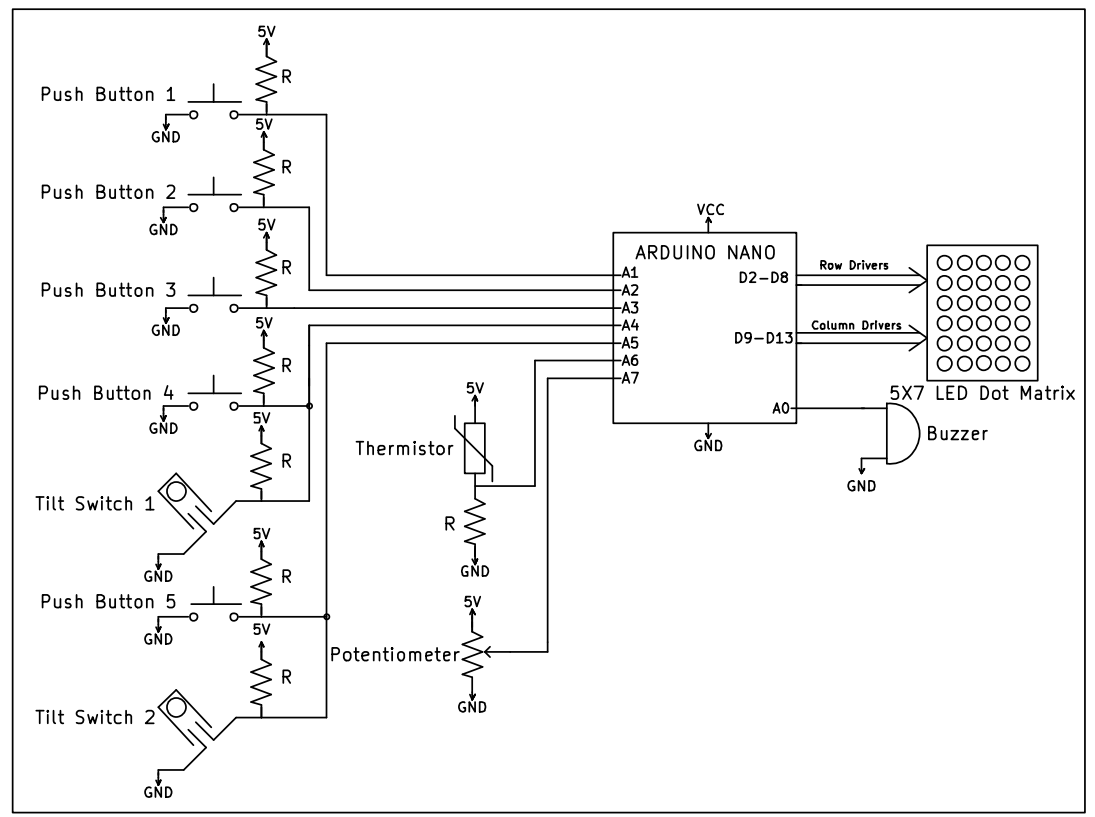
\includegraphics[width=1\textwidth]{images/Block_diagram.png}
  \caption{Block diagram}
  \label{fig:block}
\end{figure}

\subsection{Schematic Diagram}
\begin{figure}[H]
  \centering
  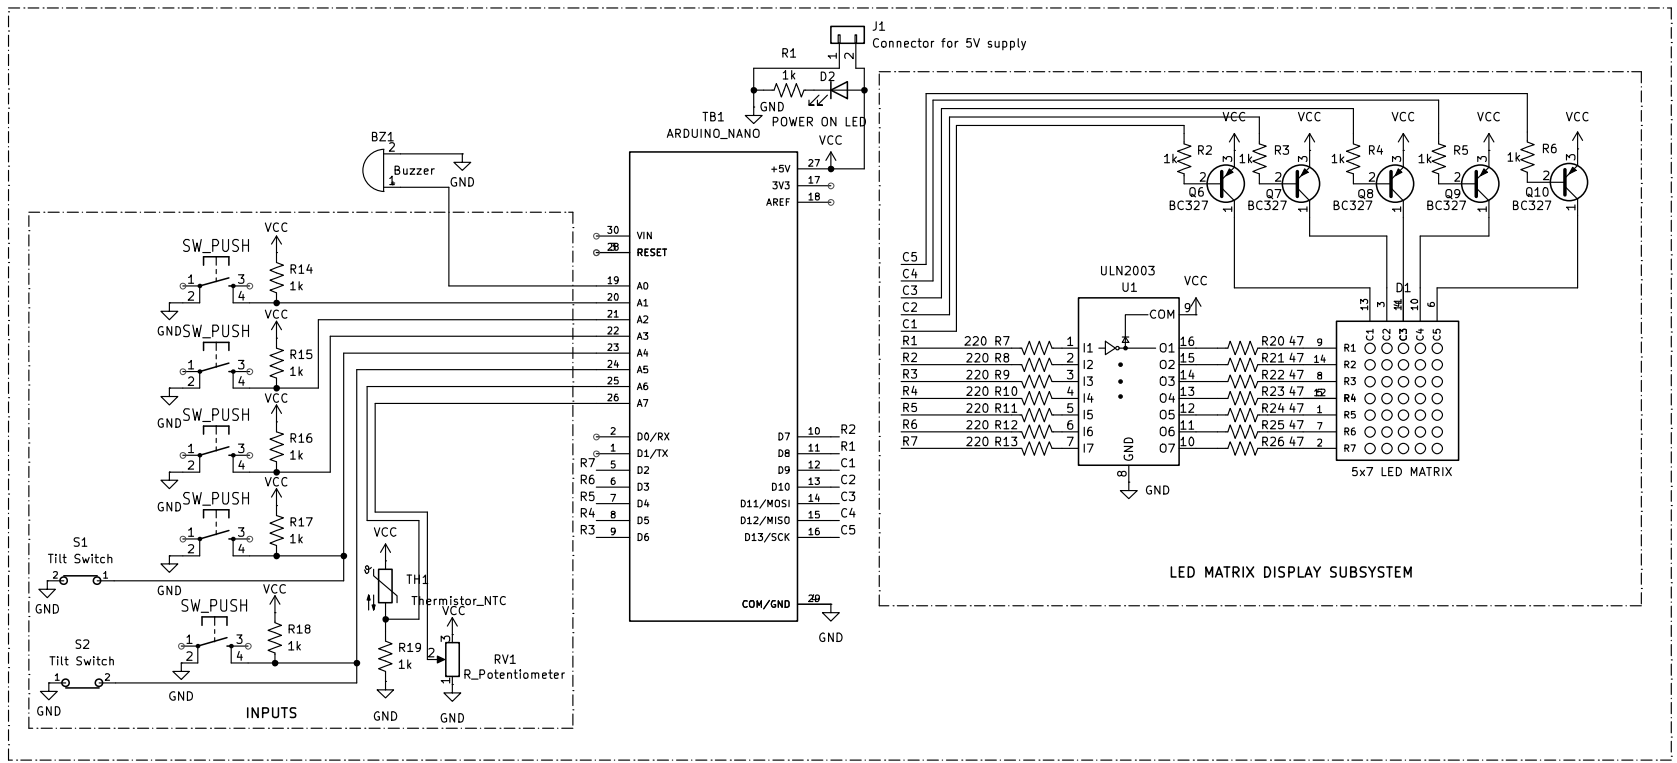
\includegraphics[width=1.4\textwidth,angle=90]{images/schematic_diagram.png}
  \caption{Schematic Diagram}
  \label{fig:schematic}
\end{figure}
%=========================================================
\subsection{Pin Assignment Table}

Table~\ref{tab:pinout} summarizes the Arduino Nano pin assignments and their corresponding peripherals used in the 4-in-1 LED Matrix Board.

\begin{table}[H]
\centering
\caption{Arduino Nano Pin Assignment}
\label{tab:pinout}
\renewcommand{\arraystretch}{1.2}
\begin{tabular}{cllp{6.5cm}}
\toprule
\textbf{Pin} & \textbf{Signal} & \textbf{Connected To} & \textbf{Function} \\
\midrule

D2  & R7 & ULN2003 IN7 & Drives Row 7 of the LED matrix \\
D3  & R6 & ULN2003 IN6 & Drives Row 6 of the LED matrix \\
D4  & R5 & ULN2003 IN5 & Drives Row 5 of the LED matrix \\
D5  & R4 & ULN2003 IN4 & Drives Row 4 of the LED matrix \\
D6  & R3 & ULN2003 IN3 & Drives Row 3 of the LED matrix \\
D7  & R2 & ULN2003 IN2 & Drives Row 2 of the LED matrix \\
D8  & R1 & ULN2003 IN1 & Drives Row 1 of the LED matrix \\

D9  & C1 & Matrix Column 1 & Column drive through BC327 transistor \\
D10 & C2 & Matrix Column 2 & Column drive through BC327 transistor \\
D11 & C3 & Matrix Column 3 & Column drive through BC327 transistor \\
D12 & C4 & Matrix Column 4 & Column drive through BC327 transistor \\
D13 & C5 & Matrix Column 5 & Column drive through BC327 transistor \\

A0 & -- & Not Used & Reserved / unused \\

A1 & BTN1 & Push Button 1 & Home navigation (Next) \\
A2 & BTN2 & Push Button 2 & Home navigation (Previous) \\
A3 & BTN3 & Push Button 3 & Home navigation (Select) \\
A4 & Tilt 1 & Tilt Switch S1/ Push Button 4 & Hourglass tilt input \\
A5 & Tilt 2 & Tilt Switch S2/ Push Button 5 & Reverse hourglass tilt input \\
A6 & Thermistor & NTC Thermistor & Temperature sensing \\
A7 & Potentiometer & RV1 & Controls POV display speed \\

5V & VCC & All peripherals & Supply voltage \\
GND & GND & Entire circuit & Common ground \\

\bottomrule
\end{tabular}
\end{table}
% =========================================================
\section{Program Logic}
\begin{figure}[H]
  \centering
  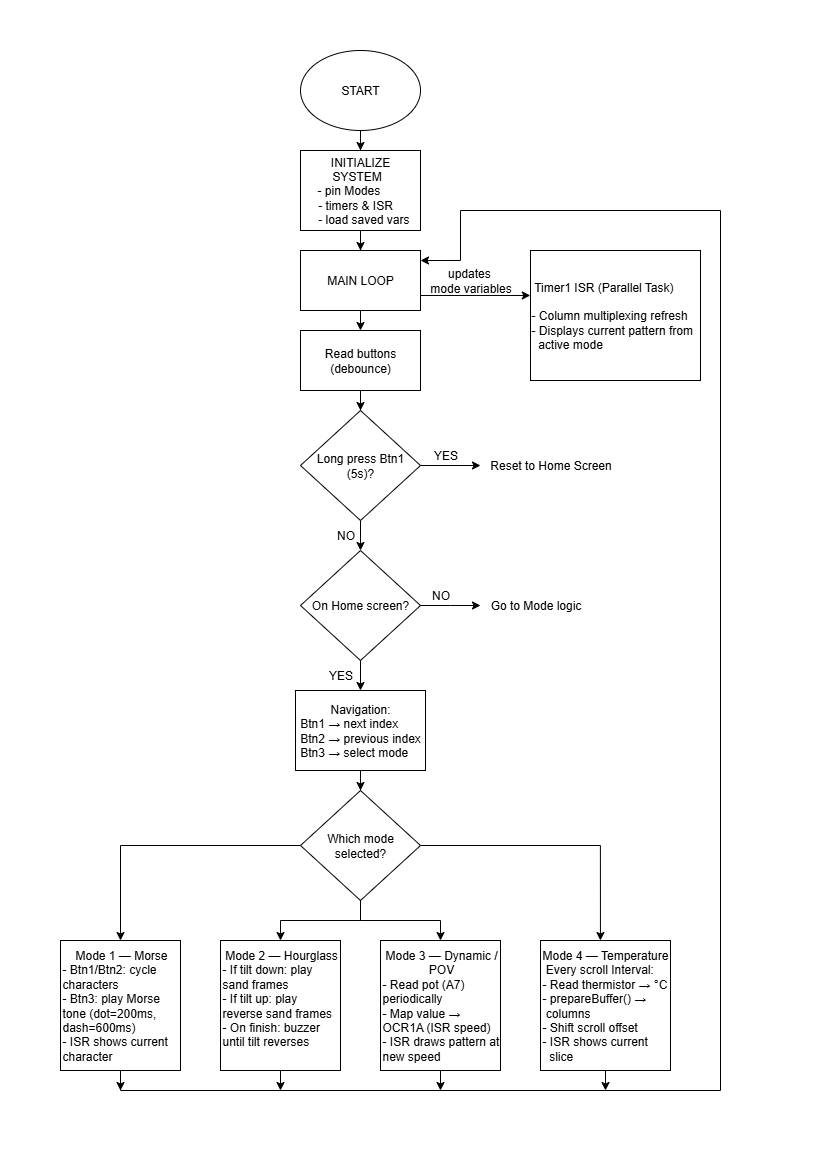
\includegraphics[width=0.9\linewidth]{images/flowchart.png}
  \caption{High-level program flowchart showing initialization, main loop logic, and Timer1 ISR operation.}
\end{figure}
\newpage
After power-up or reset, the firmware configures all GPIO pins, initializes global variables, computes the timing parameters required for animation modes, and configures \textbf{Timer1} in \textbf{Clear Timer on Compare (CTC)} mode. Timer1 generates periodic interrupts that continuously refresh the LED matrix using column-wise multiplexing, allowing the main program to execute application logic independently of display updates.

The firmware follows a cooperative architecture consisting of a foreground \textbf{main loop} and a background \textbf{Timer1 Interrupt Service Routine (ISR)}. The main loop is responsible for processing user inputs, updating mode-specific variables, and preparing display data, while the ISR performs high-speed multiplexing of the LED matrix to maintain a stable, flicker-free display.

The overall firmware operation is summarized below.

\begin{enumerate}[itemsep=4pt]

\item \textbf{Home Screen Navigation:}
When no application mode is active, the LED matrix displays the home screen. Three push buttons are used for menu navigation:
\begin{itemize}
    \item Button~1 -- Next mode
    \item Button~2 -- Previous mode
    \item Button~3 -- Select mode
\end{itemize}
A long press of Button~1 (approximately 5\,s) exits any running mode and returns the system to the home screen.

\item \textbf{Mode Execution:}
After a mode is selected, the corresponding application logic executes within the main loop.
\begin{itemize}
    \item \textbf{Mode 1:} Morse Tutor
    \item \textbf{Mode 2:} LED Hourglass
    \item \textbf{Mode 3:} Persistence of Vision (POV) Demo
    \item \textbf{Mode 4:} Temperature Display
\end{itemize}

\item \textbf{Background Display Refresh:}
The Timer1 ISR executes periodically throughout system operation. During each interrupt, one column of the LED matrix is refreshed by outputting the appropriate bitmap corresponding to the currently active mode. This interrupt-driven multiplexing ensures uniform brightness and prevents visible display flicker.

\item \textbf{Foreground Processing:}
While the ISR refreshes the display, the main loop continuously performs button debouncing, tilt-switch monitoring, potentiometer and thermistor acquisition, mode transitions, animation control, and updates the display buffer whenever the displayed content changes.

\end{enumerate}
\newpage
% =========================================================
\section{Inputs and Control Logic}
\subsection{Buttons and Navigation}

Three push buttons provide user interaction with the system. Each button is configured using the Arduino Nano's internal \texttt{INPUT\_PULLUP} resistor, eliminating the need for external pull-down resistors and ensuring a stable default logic HIGH state. Consequently, a button press is detected as a logic LOW (active LOW).

During Home Screen operation, Button~1 and Button~2 are used to navigate through the available modes, while Button~3 selects the highlighted mode. To improve usability, the firmware also detects a long press (approximately 5\,s) on Button~1, allowing the user to exit any active mode and return directly to the Home Screen.

\subsection{Tilt Interaction}

The Hourglass mode uses two tilt switches to detect the orientation of the board. Each switch is configured as an active LOW digital input using the Arduino Nano's internal pull-up resistor. Depending on the detected orientation, the firmware determines the direction of the sand animation.

\begin{itemize}[itemsep=2pt]
    \item When the board is tilted downward, the sand animation is played in the forward direction, simulating sand falling to the bottom chamber.
    
    \item When the board is tilted upward, the animation is played in the reverse direction, simulating the hourglass being inverted.
    
    \item After the final animation frame is displayed, the passive buzzer generates an audible alert. The alert continues until the board is tilted in the opposite direction or the mode is reset.
\end{itemize}
\textbf{Note:} The tilt switches are connected to Arduino Nano pins \textbf{A4} and \textbf{A5}, which are also routed to \textbf{Button~4} and \textbf{Button~5}, respectively, on the development board. These pins are dedicated to tilt sensing in the current implementation and are therefore not used as general-purpose push buttons.

\subsection{Potentiometer and Display Refresh Control}

The Persistence of Vision (POV) mode uses a potentiometer to provide real-time control over the display refresh rate. The potentiometer output is continuously sampled through the Arduino Nano's ADC, and the measured value is used to adjust the Timer1 compare register (\texttt{OCR1A}).

Modifying the Timer1 compare value changes the interrupt period, thereby varying the LED matrix refresh frequency. At higher refresh rates, the displayed character appears stable due to the persistence-of-vision effect, whereas lower refresh rates make the row-by-row multiplexing process visible. This provides an interactive demonstration of how refresh frequency influences the perceived display.
\newpage

\subsection{Thermistor and Temperature Calculation}

Temperature measurement is performed using an NTC thermistor connected in a voltage divider configuration with a fixed \SI{1}{k\ohm} resistor. The Arduino Nano measures the divider voltage using its ADC, from which the thermistor resistance is calculated. The resistance is then converted into temperature using the \textbf{Beta parameter model}, which provides a good balance between computational simplicity and measurement accuracy for NTC thermistors.

The thermistor resistance is calculated as

\[
R_\mathrm{th}=R_\mathrm{pullup}\frac{5-V}{V},
\]

where \(V\) is the measured divider voltage.

The temperature in Kelvin is then obtained using

\[
T(K)=
\frac{1}
{\dfrac{1}{T_0}+
\dfrac{1}{\beta}
\ln\left(\dfrac{R_\mathrm{th}}{R_0}\right)},
\]

where

\[
T_0=298.15~\mathrm{K}, \qquad
\beta=3950, \qquad
R_0=\SI{1}{k\ohm}, \qquad
R_\mathrm{pullup}=\SI{1}{k\ohm}.
\]

The calculated temperature is converted to degrees Celsius and formatted into a scrolling text buffer using the \texttt{prepareBuffer()} function before being displayed on the LED matrix.
\newpage

% =========================================================
\section{Working Modes}


\subsection{Home Screen}

The Home Screen serves as the primary user interface of the system. It displays five icons corresponding to the available operating modes: Home, Morse Tutor, Hourglass, Persistence of Vision (POV) Demo, and Temperature Display. Users can navigate between these icons using Button~1 and Button~2, while Button~3 selects the highlighted mode. A long press of Button~1 returns the system to the Home Screen from any active mode.

\begin{figure}[H]
  \centering
  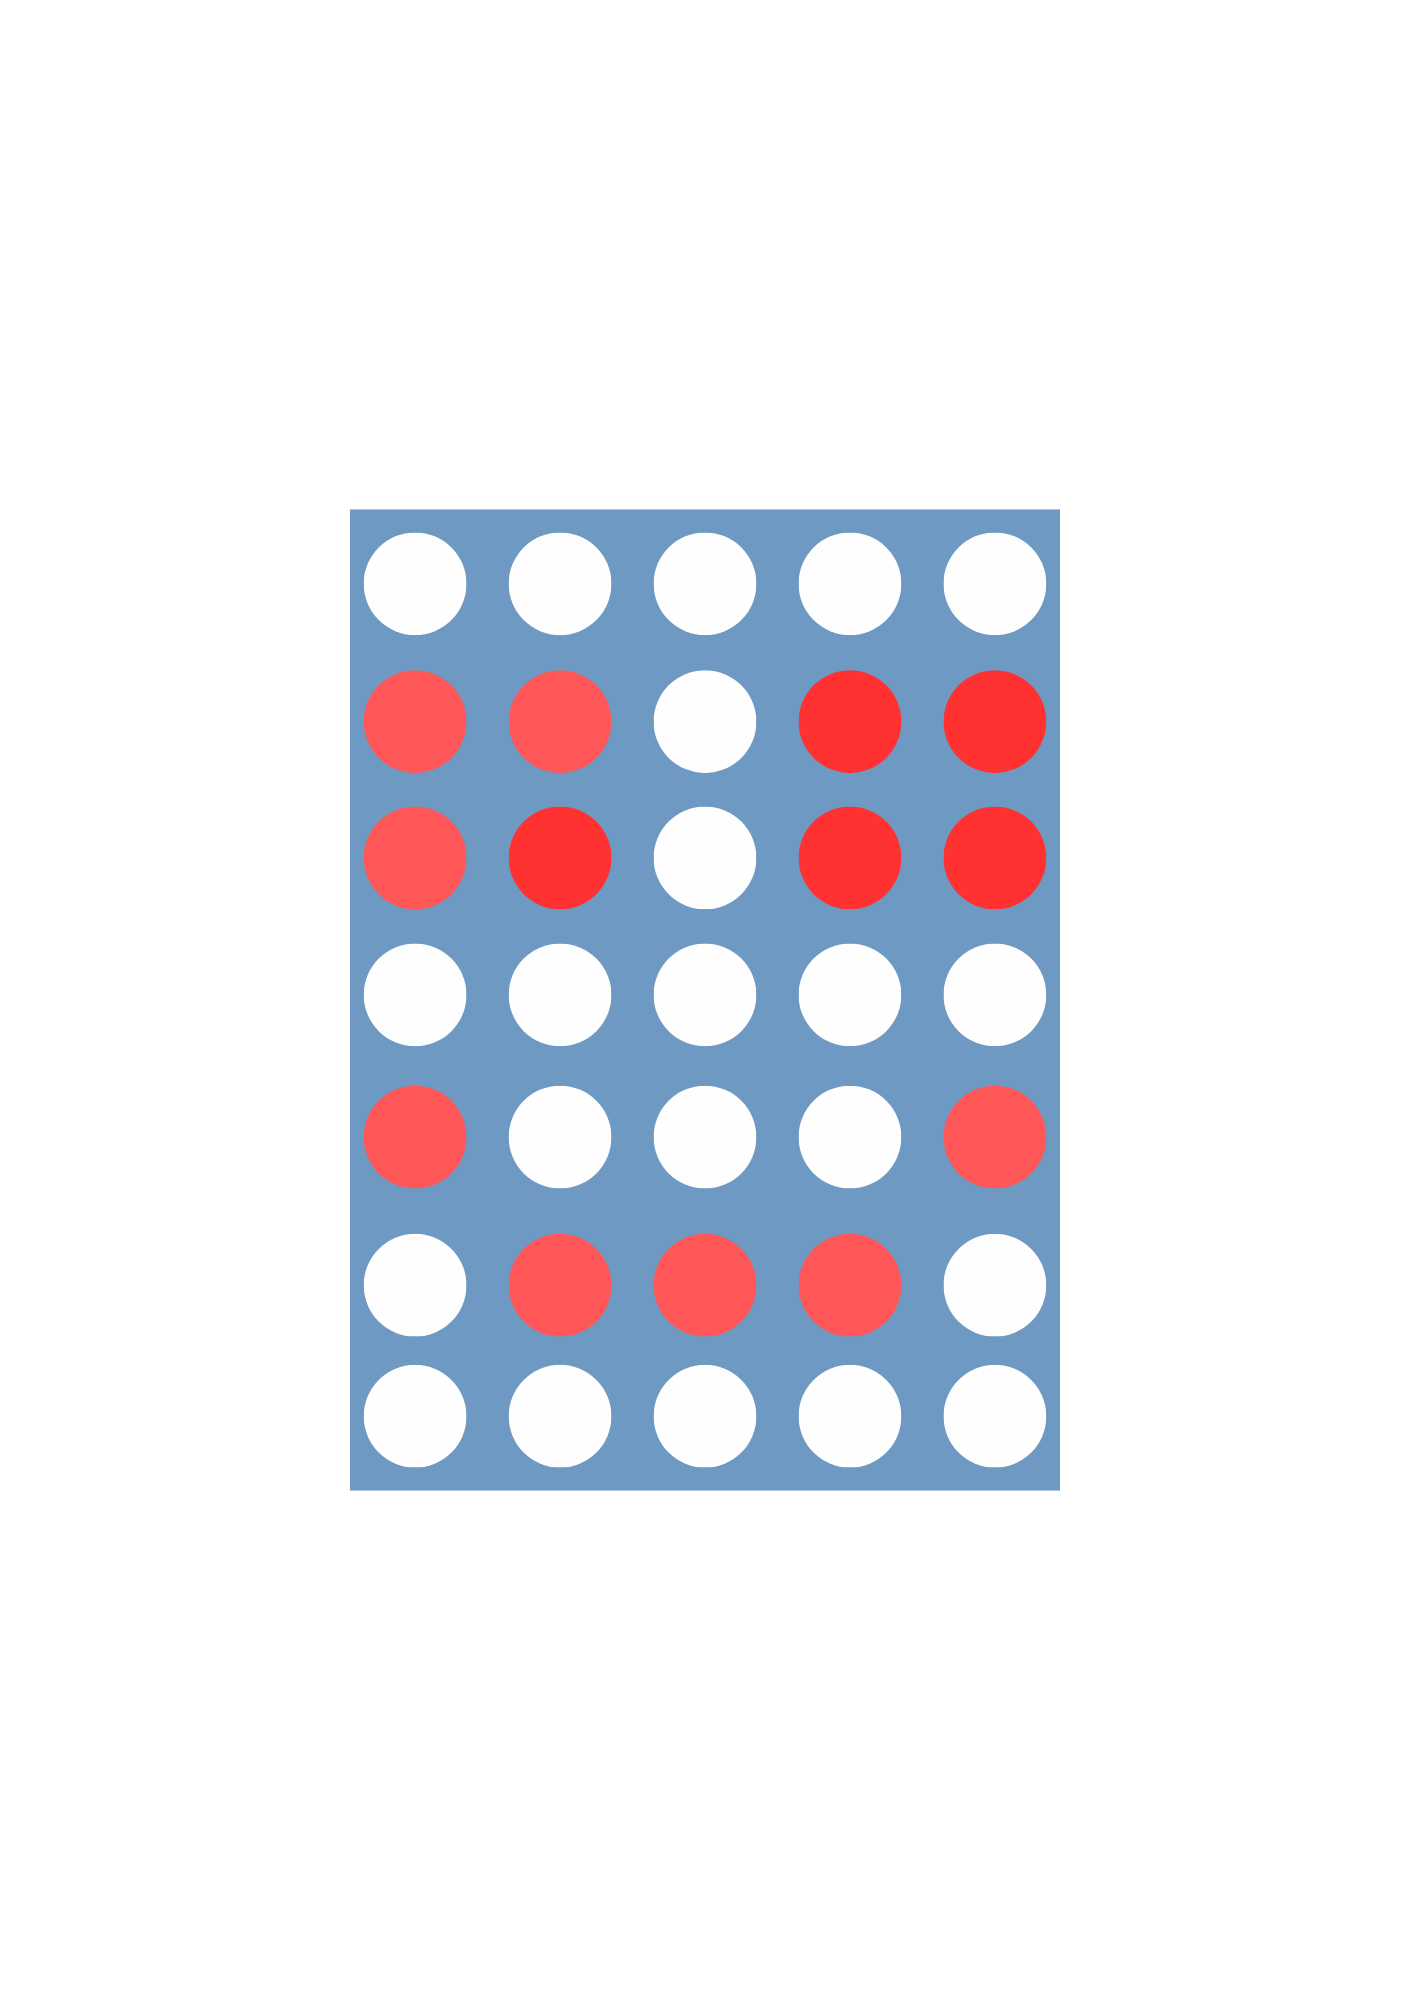
\includegraphics[width=0.6\textwidth]{images/Home_Screen.png}
  \caption{Home screen icons on the 5$\times$7 matrix.}
\end{figure}
\newpage
\subsection{Mode 1: Morse Tutor}

\begin{itemize}[itemsep=2pt]

\item \textbf{Selection:} Buttons~1 and~2 are used to cycle through the supported alphanumeric characters (A--Z and 0--9). Button~3 transmits the selected character as Morse code.

\item \textbf{Operation:} Each character is encoded according to the International Morse Code standard. A dot is represented by a \SI{200}{ms} tone, while a dash is represented by a \SI{600}{ms} tone. The corresponding sequence is generated through the onboard passive buzzer.

\item \textbf{Display:} The selected character is simultaneously displayed on the 5$\times$7 LED matrix, allowing users to associate the visual character with its corresponding Morse code representation.

\end{itemize}

\begin{figure}[H]
  \centering
  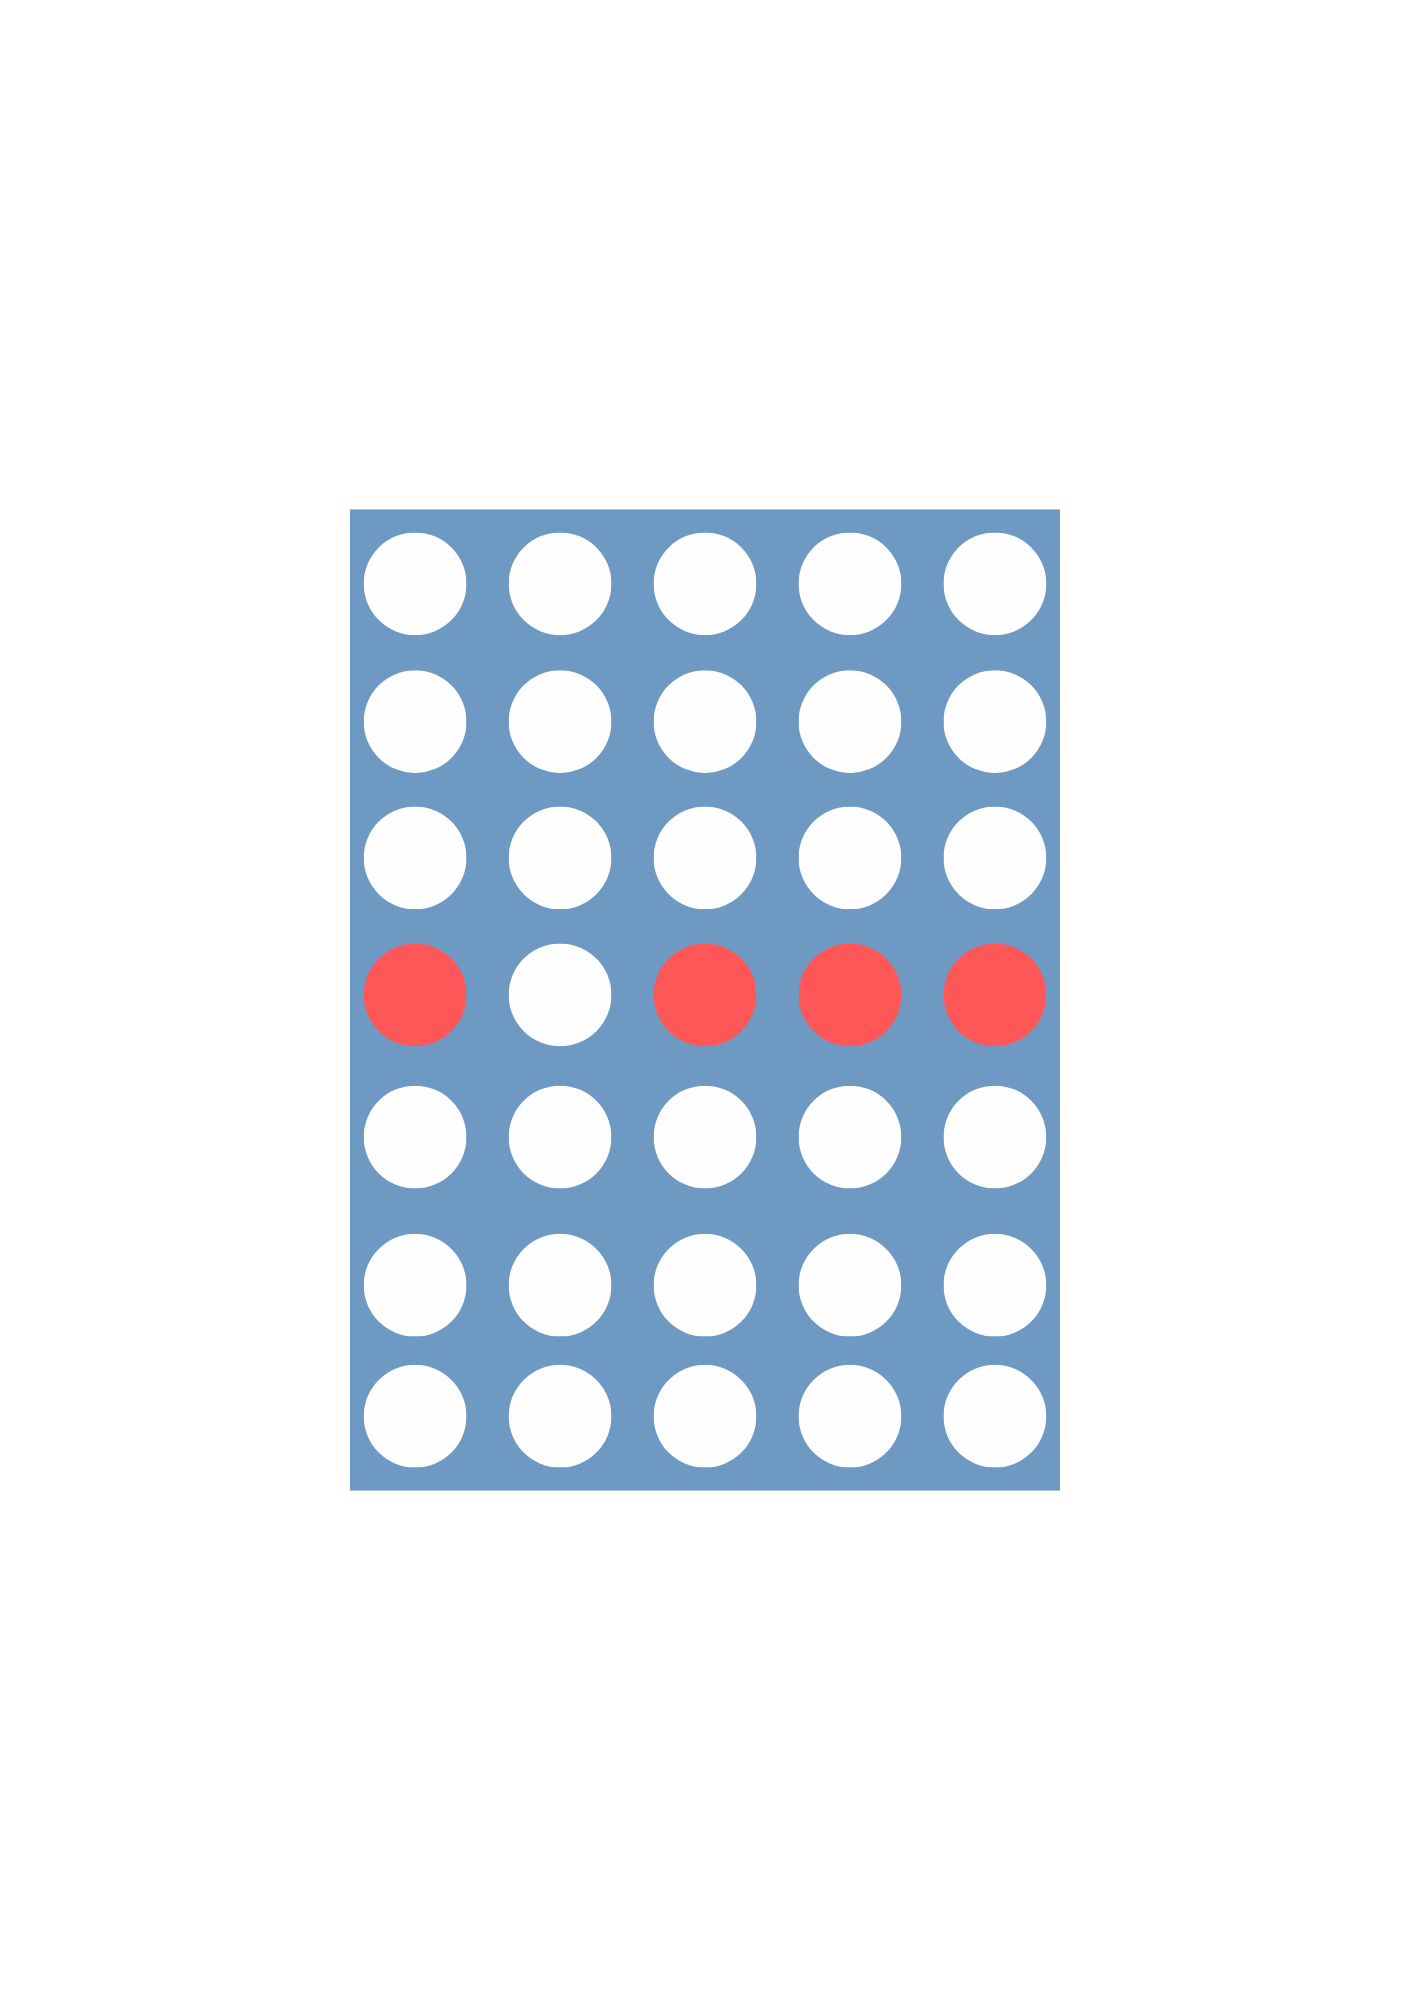
\includegraphics[width=0.6\textwidth]{images/Morse_Tutor.png}
  \caption{Morse Tutor mode glyph preview.}
\end{figure}
\newpage
\subsection{Mode 2: Hourglass}
\begin{itemize}[itemsep=2pt]

\item \textbf{Animation:} The LED matrix displays a sequence of pre-defined bitmap frames that simulate sand flowing between the two chambers of an hourglass.

\item \textbf{Control:} Two tilt switches detect the orientation of the board. Tilting the board upward or downward causes the animation to play in the corresponding direction, emulating the inversion of a physical hourglass.

\item \textbf{Alert:} Once the animation reaches its final frame, the passive buzzer generates a continuous audible alert. The alert remains active until the board is tilted in the opposite direction or the mode is reset.

\end{itemize}

\begin{figure}[H]
  \centering
  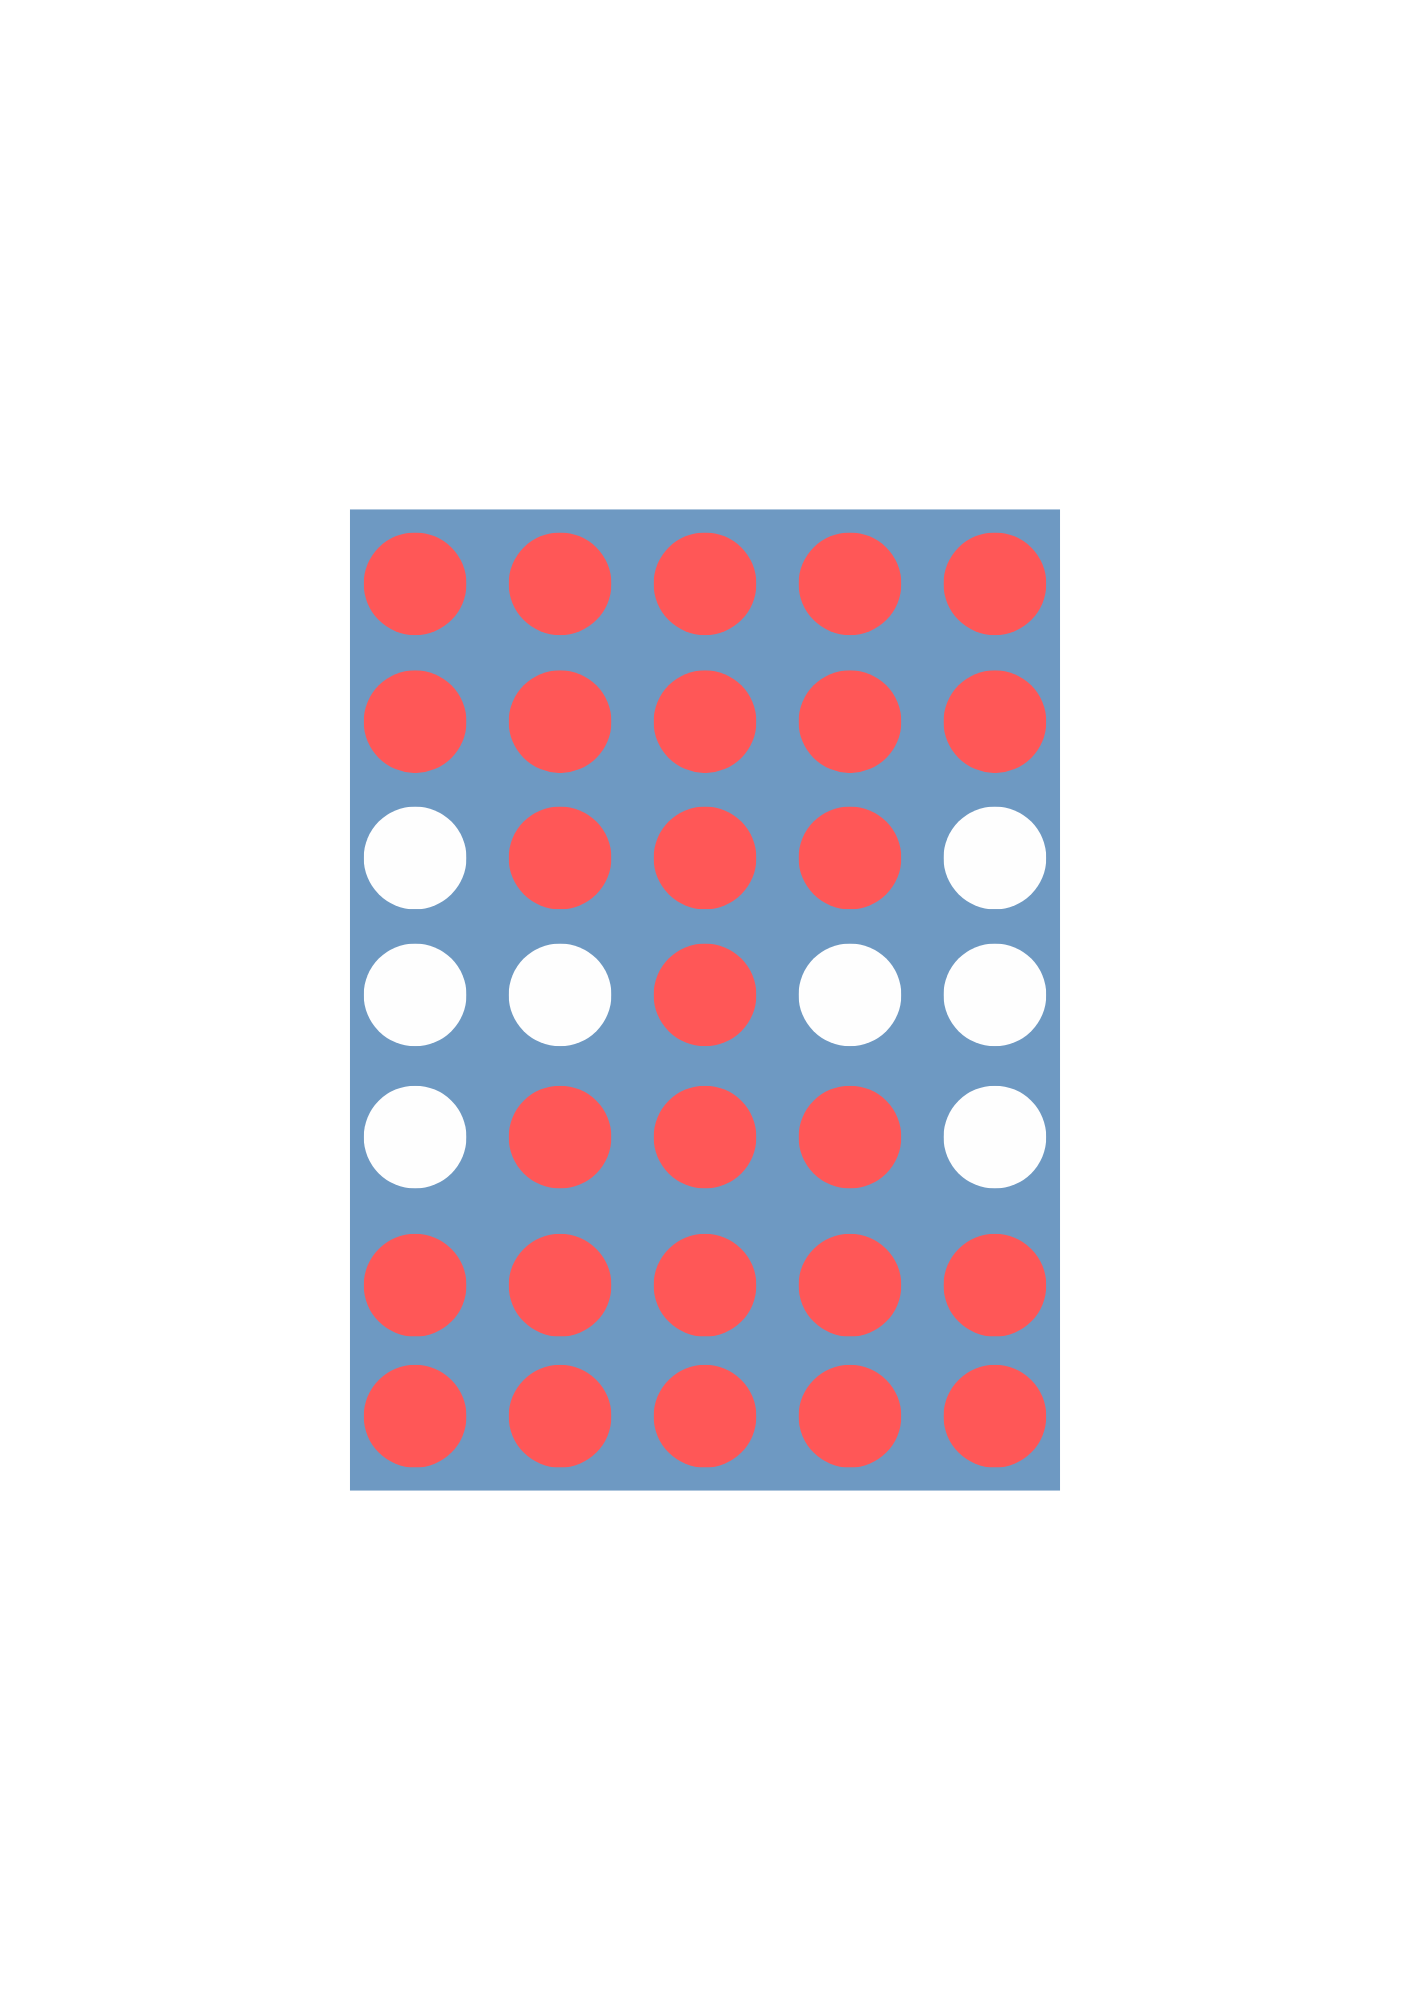
\includegraphics[width=0.6\textwidth]{images/Hour_Glass.png}
  \caption{Hourglass mode glyph preview.}
\end{figure}
\newpage
\subsection{Mode 3: POV Demo}
\begin{itemize}[itemsep=2pt]

\item \textbf{Concept:} This mode demonstrates the principle of Persistence of Vision (POV), where the LED matrix is refreshed at a sufficiently high frequency to create the perception of a stable, continuous image.

\item \textbf{Control:} The display refresh rate is controlled using a potentiometer. By varying the Timer1 interrupt period, the user can adjust the matrix scanning speed, allowing the transition from a flicker-free display to visible row-by-row multiplexing to be observed.

\item \textbf{Display:} A demonstration character is displayed on the LED matrix to illustrate the persistence-of-vision effect. The displayed bitmap can be replaced with any user-defined pattern.

\end{itemize}

\begin{figure}[H]
  \centering
  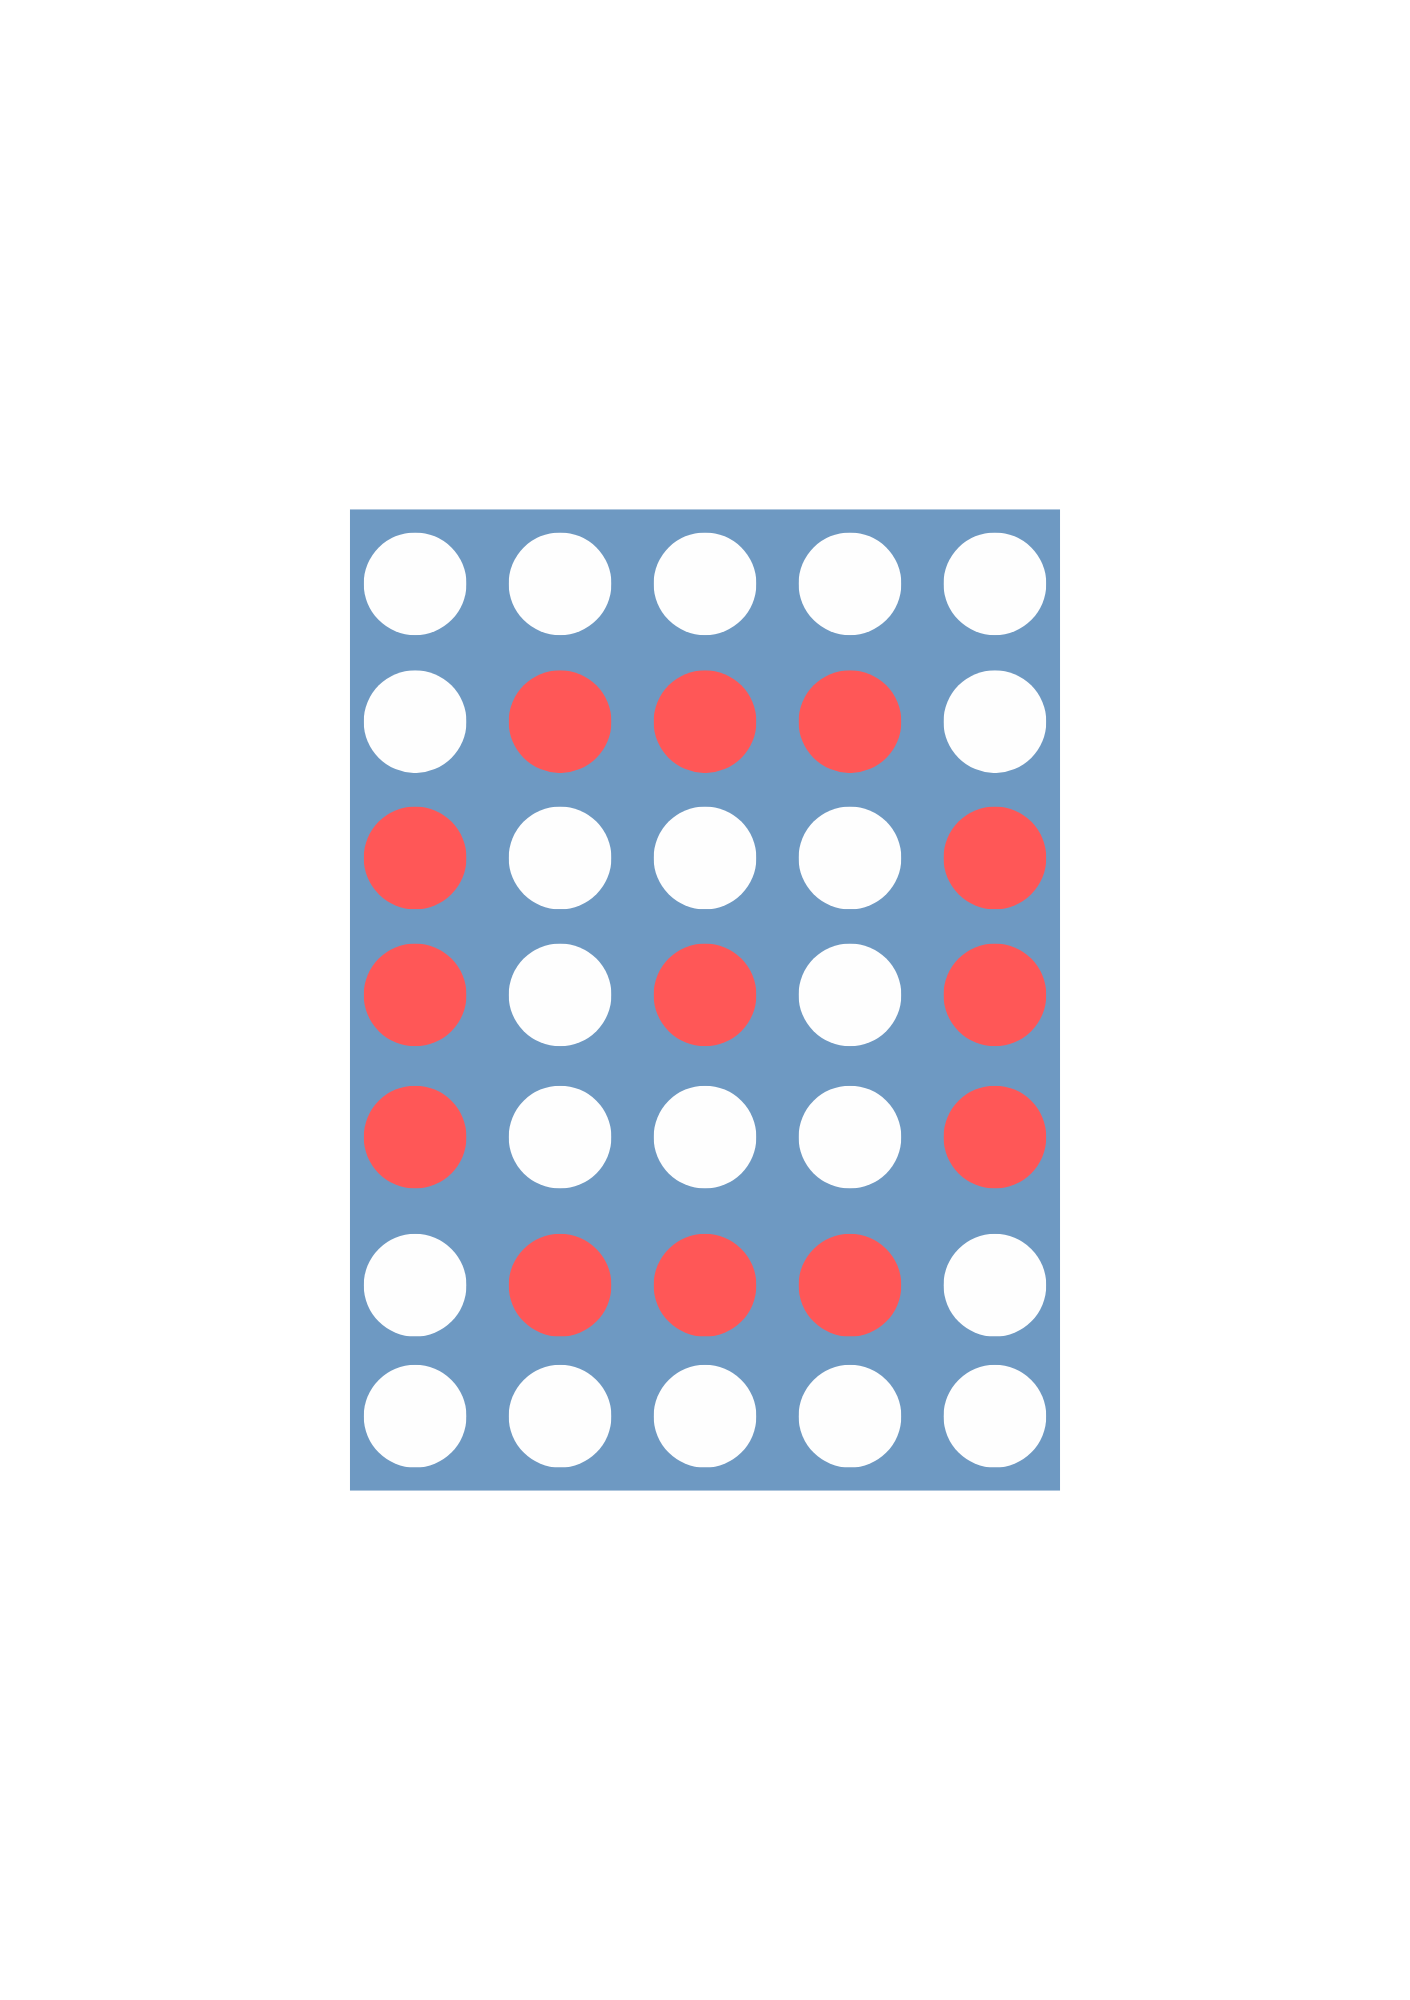
\includegraphics[width=0.6\textwidth]{images/POV_Demo.png}
  \caption{POV Demo mode glyph preview.}
\end{figure}
\newpage
\subsection{Mode 4: Temperature Display}
\begin{itemize}[itemsep=2pt]

\item \textbf{Acquisition:} The thermistor is periodically sampled using the Arduino Nano's analog-to-digital converter (ADC). The measured voltage is converted into temperature using the Beta parameter model described in Section~5.4.

\item \textbf{Rendering:} The calculated temperature is formatted as a text string and converted into a bitmap representation suitable for display on the 5$\times$7 LED matrix.

\item \textbf{Scrolling:} Since the display is limited to five columns, the temperature is presented as a horizontally scrolling message, allowing the complete value to be viewed continuously.

\end{itemize}

\begin{figure}[H]
  \centering
  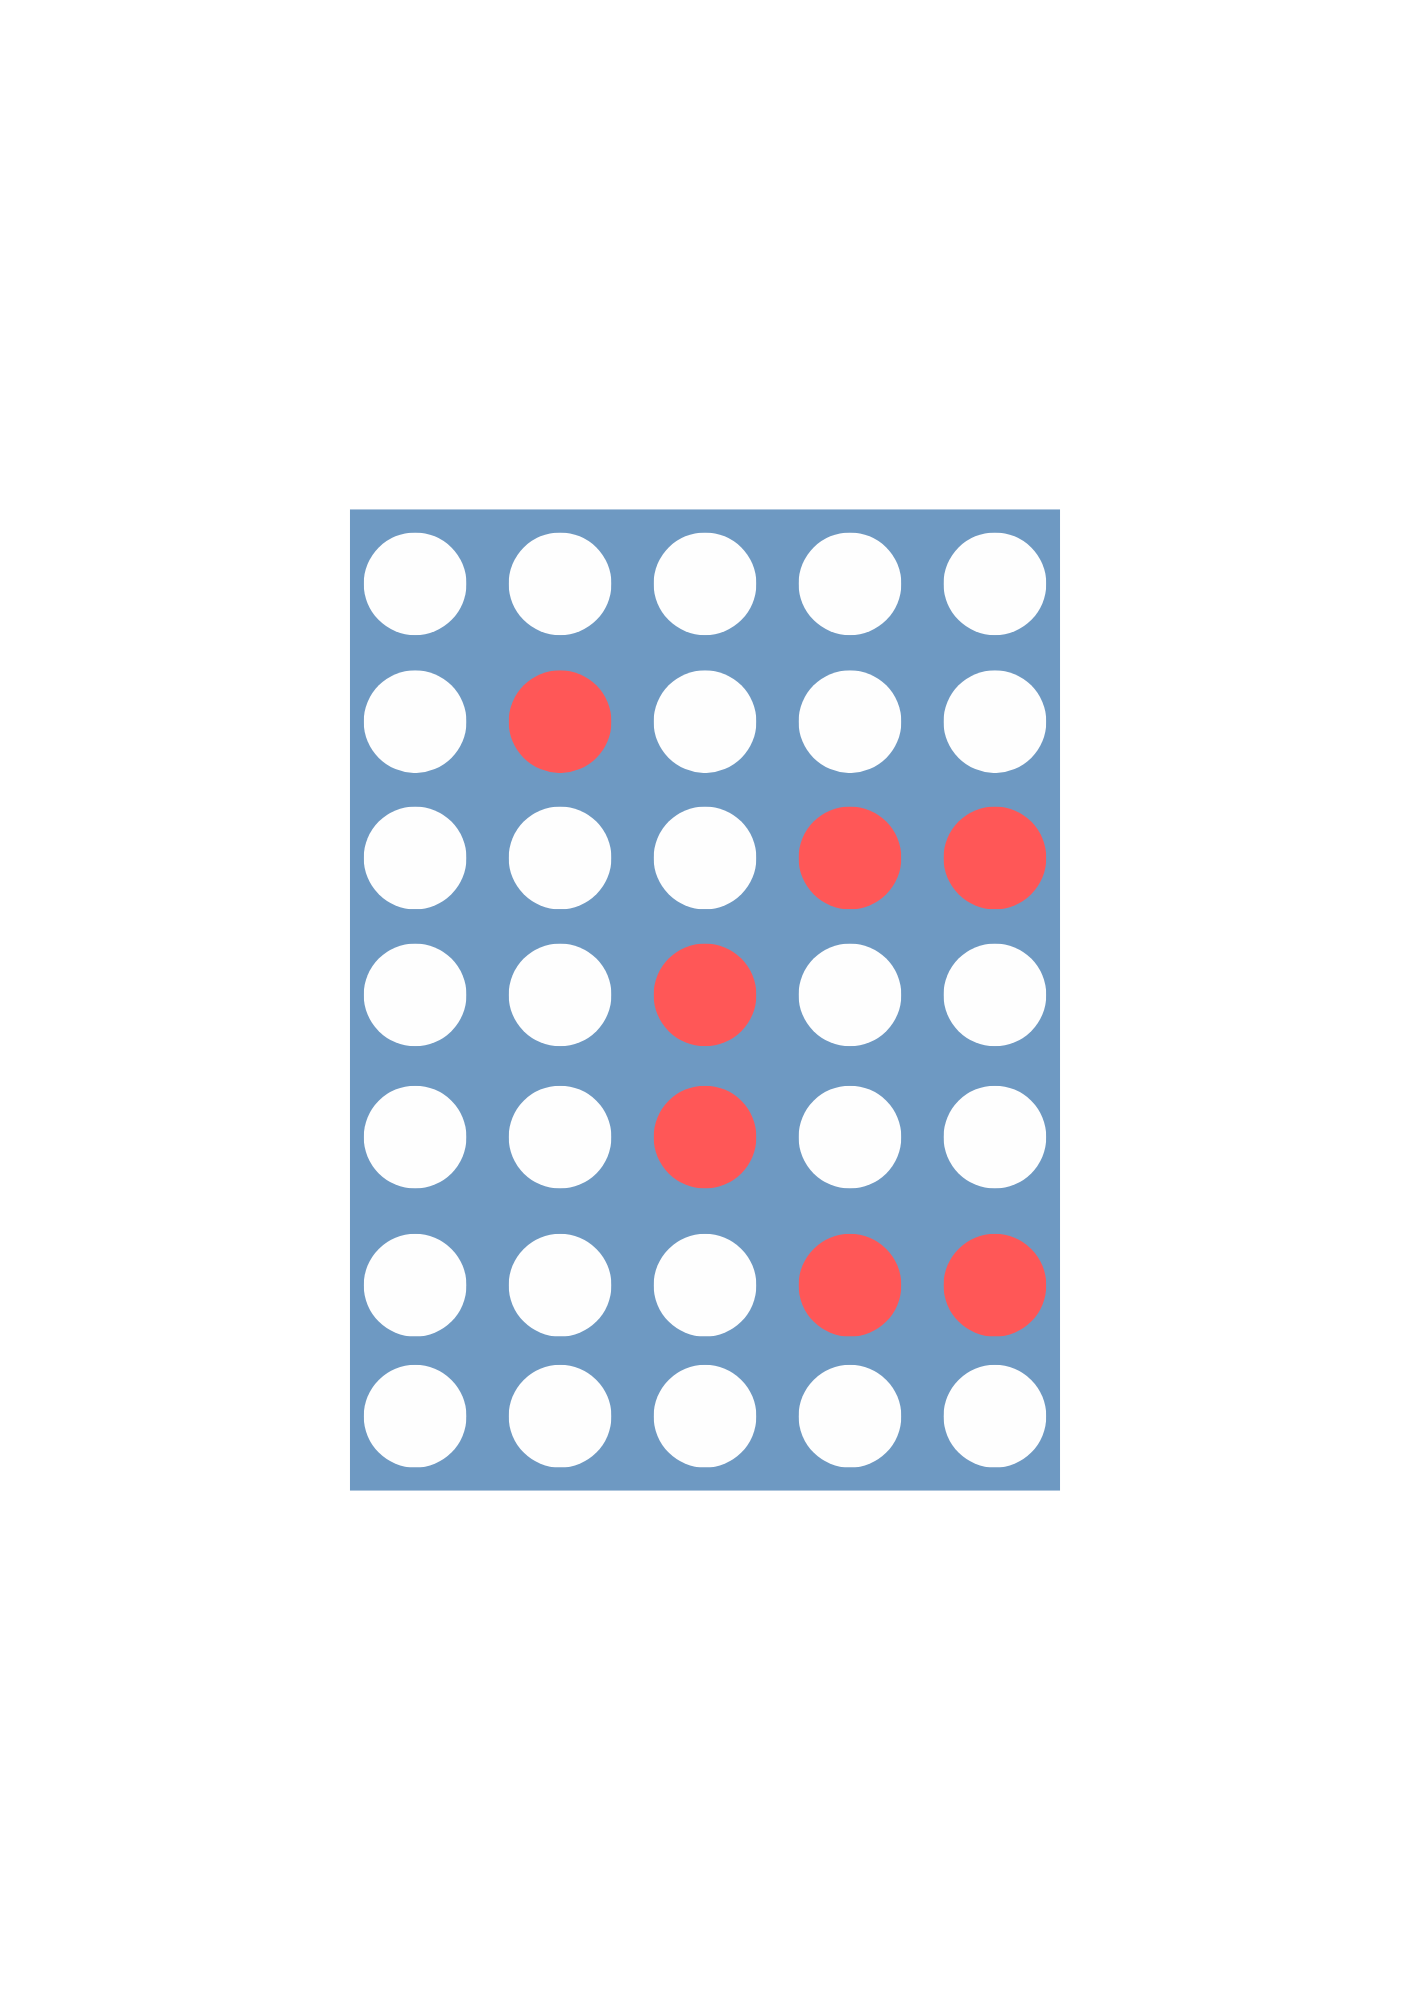
\includegraphics[width=0.6\textwidth]{images/Temperature_Display.png}
  \caption{Temperature Display mode glyph preview.}
\end{figure}
\newpage

\section{Bill Of Material(BOM)}

\begin{figure}[H]
  \centering
  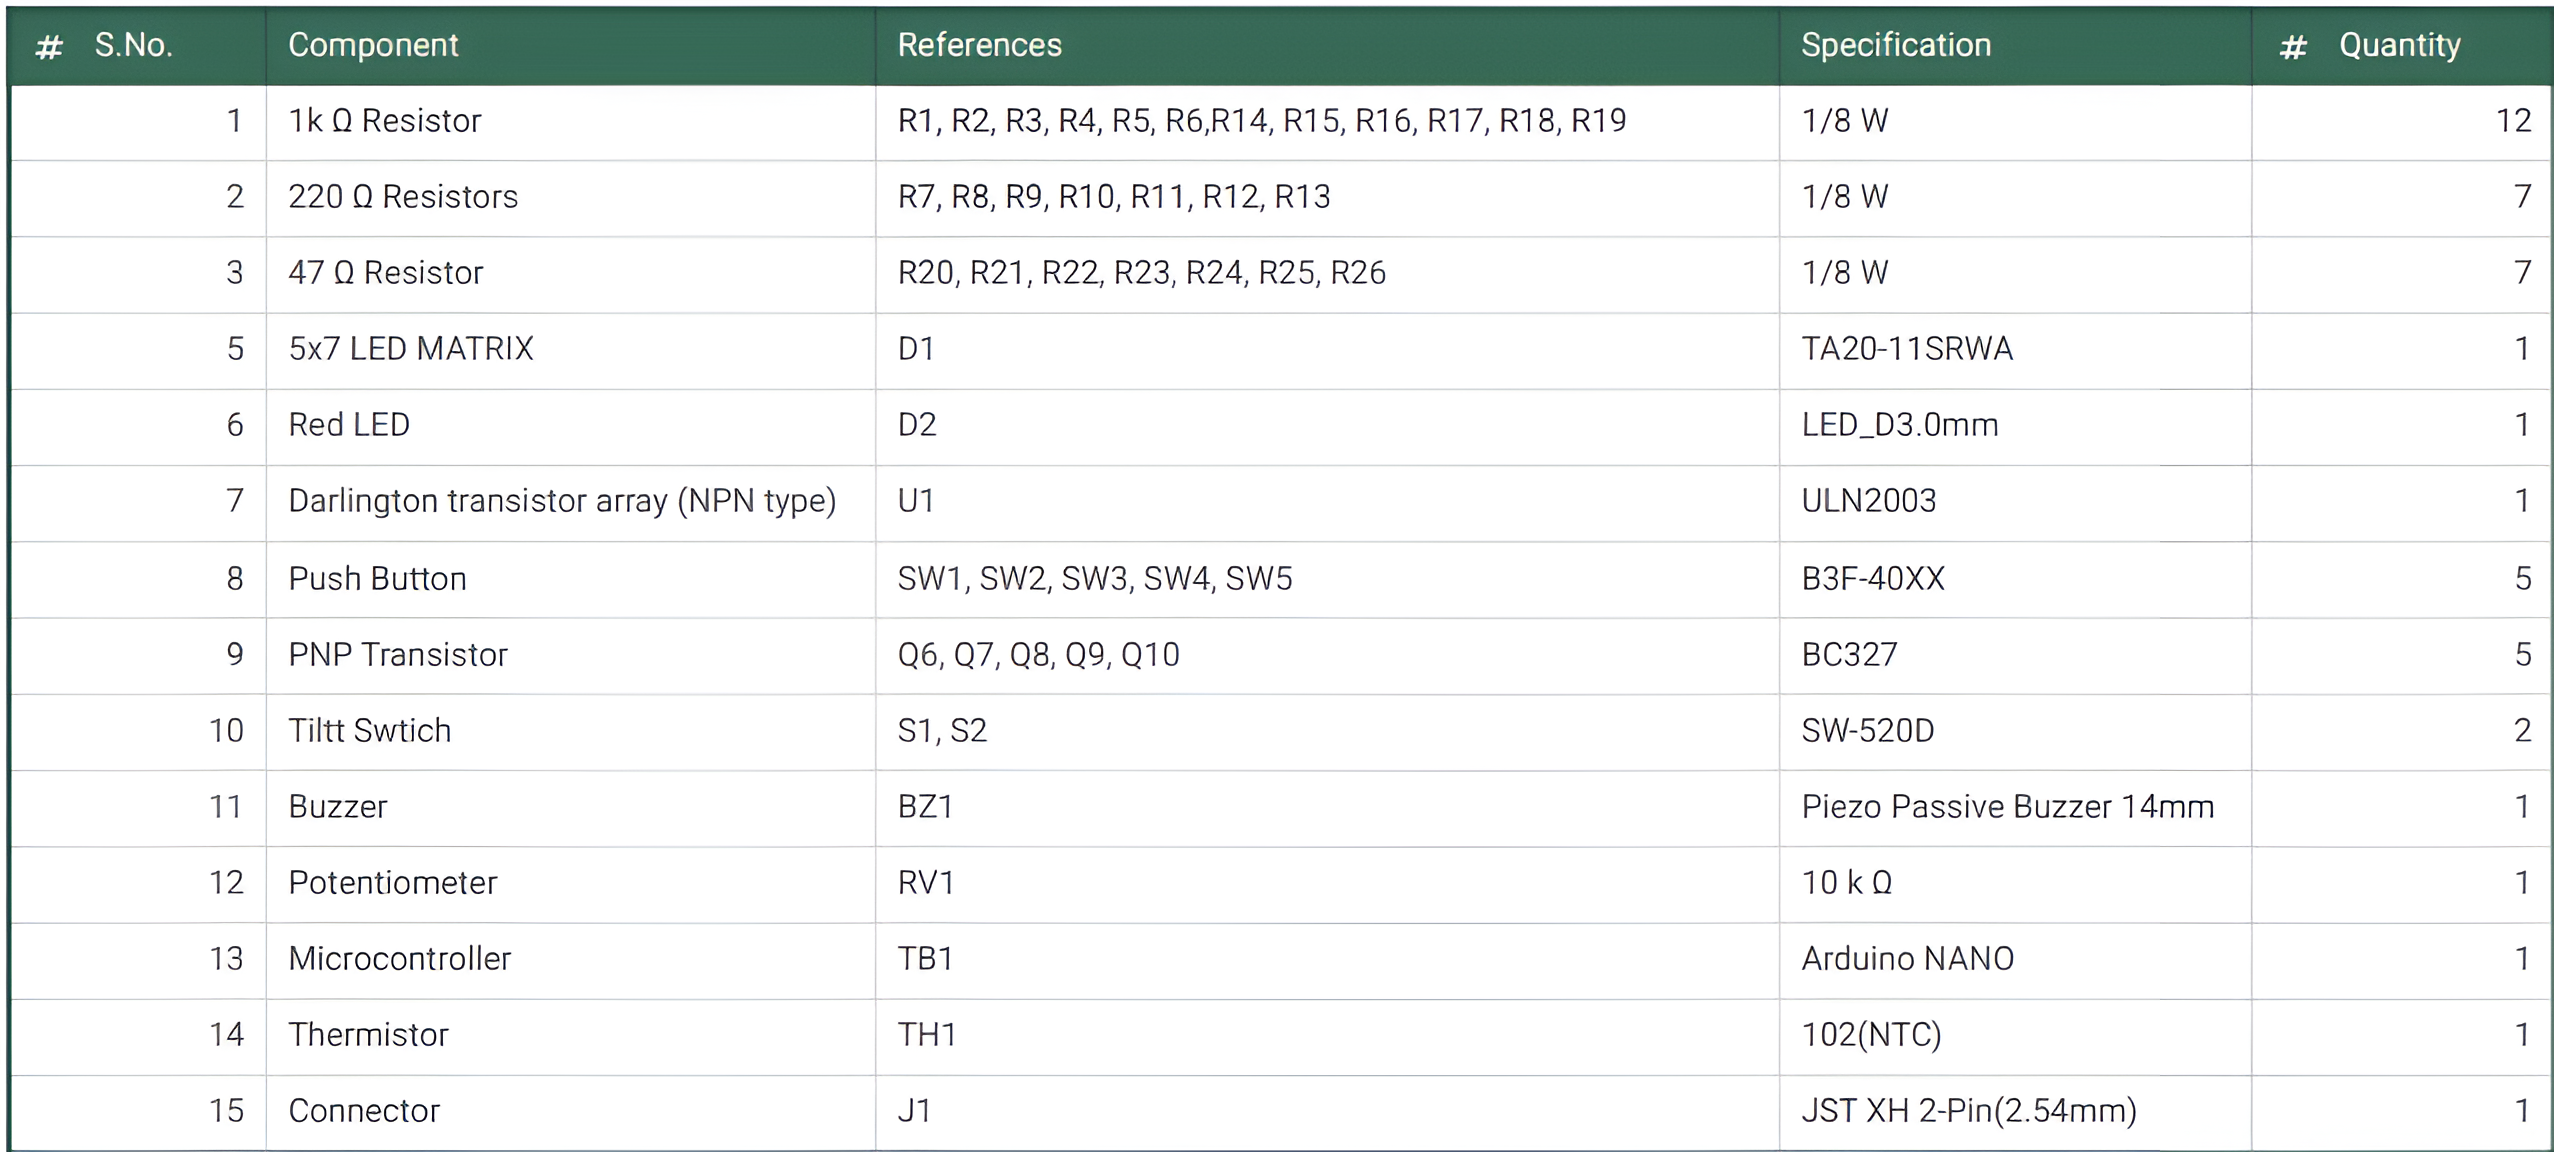
\includegraphics[width=1
  \textwidth]{images/BOM.png}
  \caption{Bill of Material}
\end{figure}
\newpage
% =========================================================
\section{Result}
\begin{figure}[H]
  \centering
  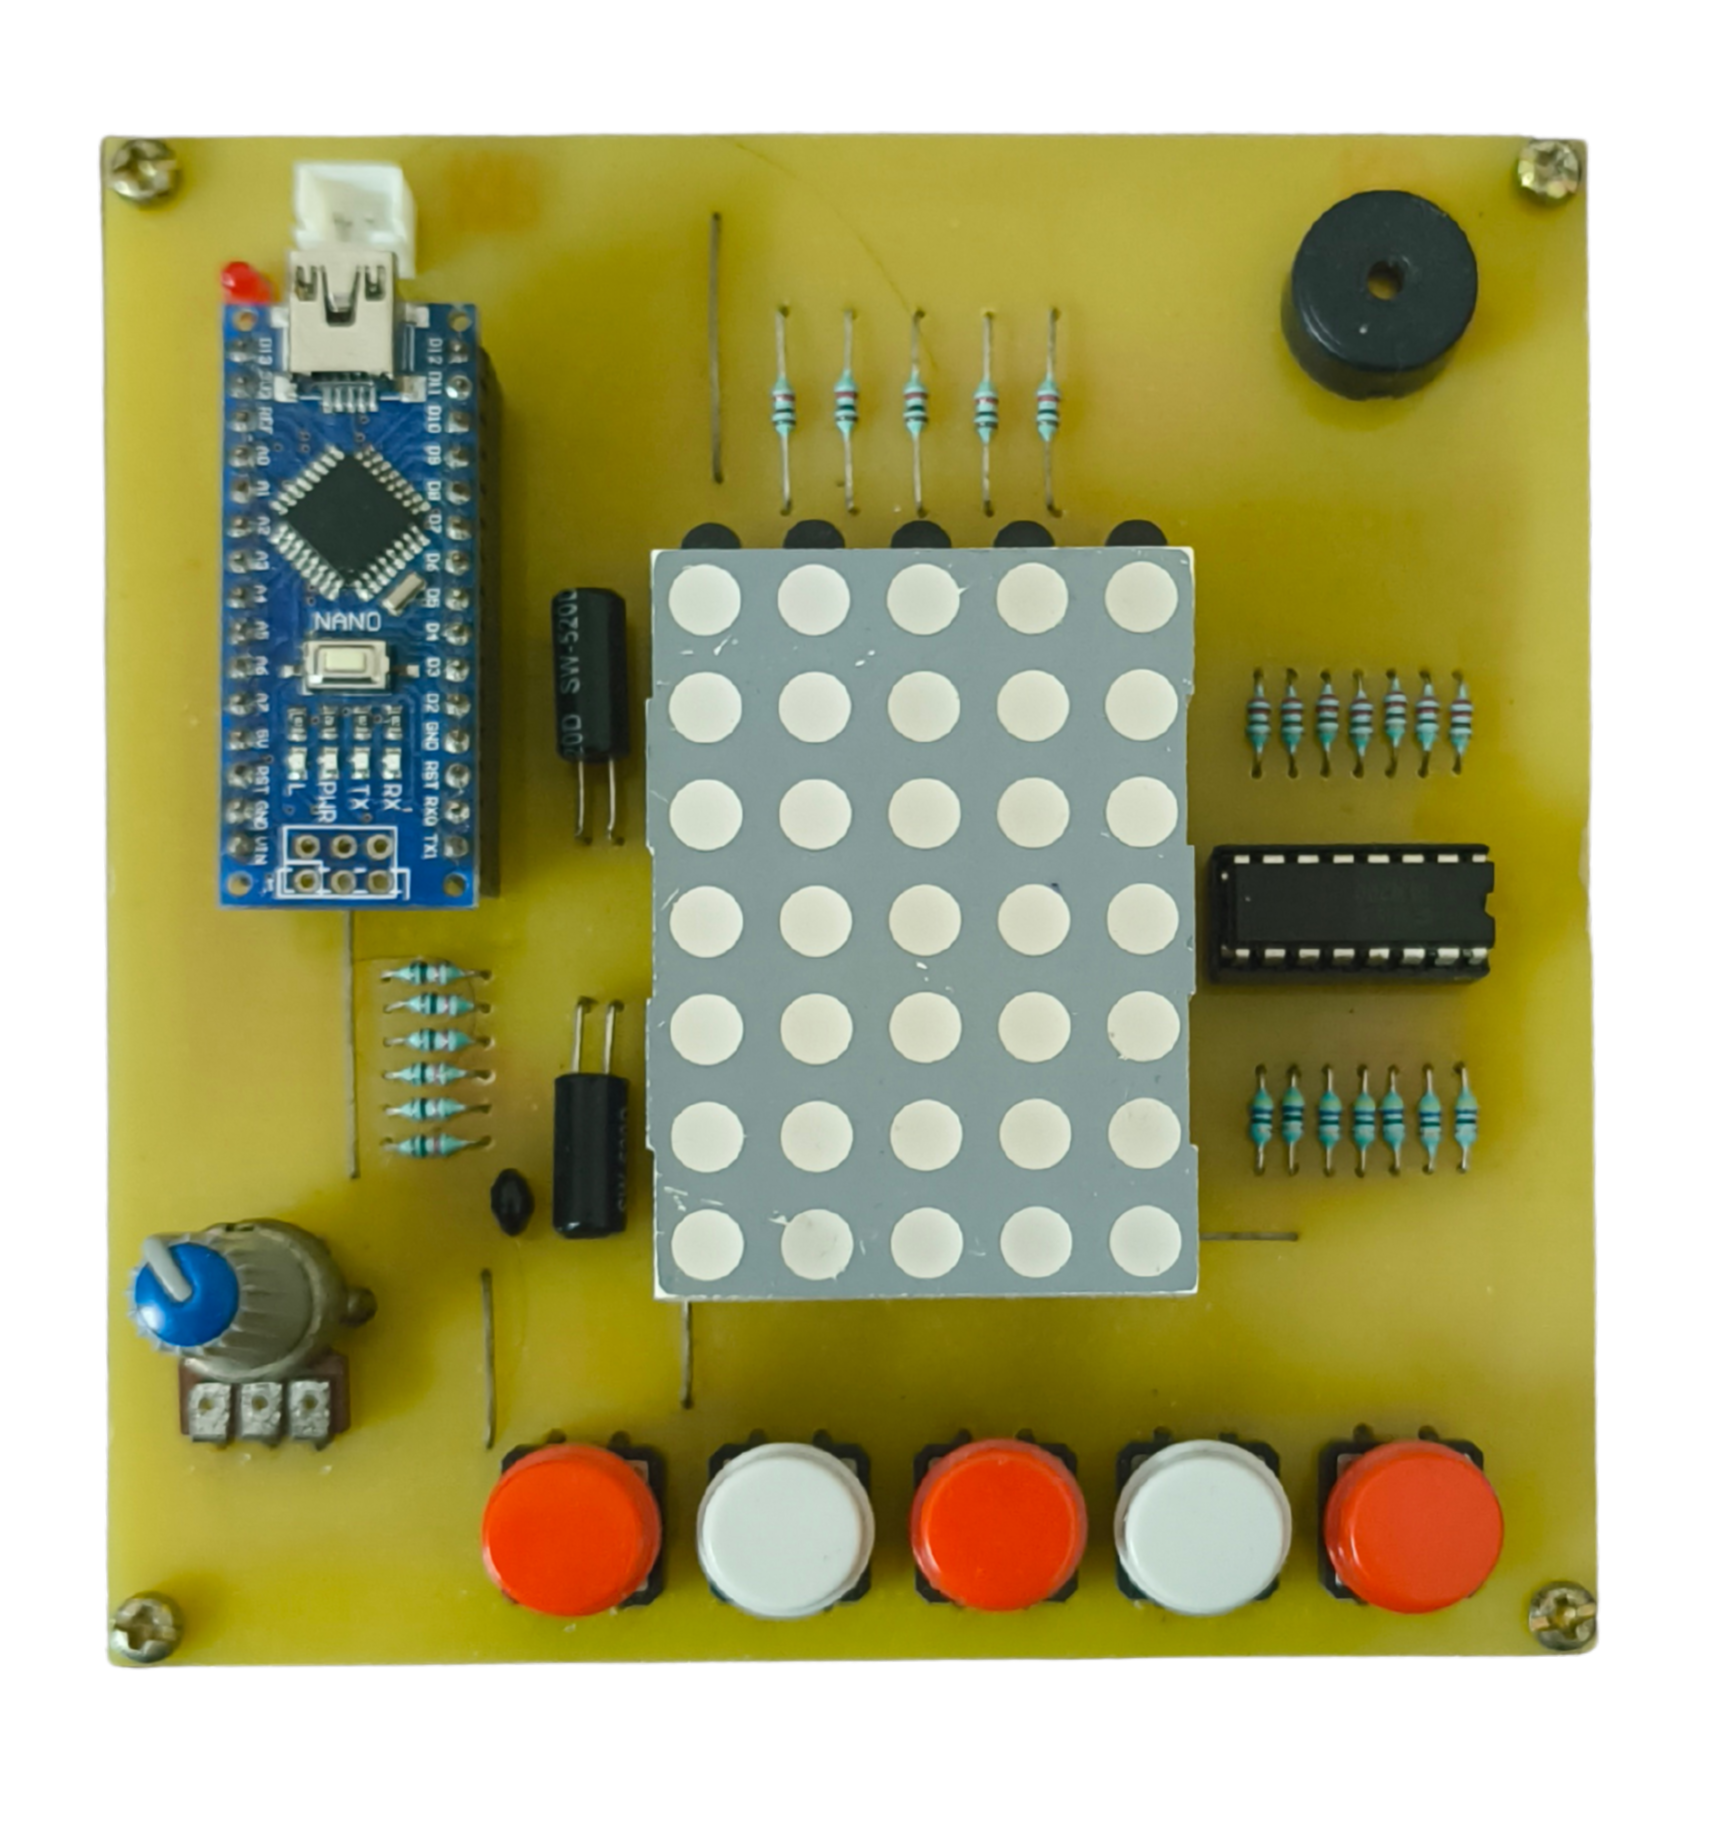
\includegraphics[width=0.8\textwidth]{images/board.png}
  \caption{4-in-1 LED Matrix Board}
\end{figure}
% =========================================================


% =========================================================
\section*{Appendix}


\subsection*{Code Files}
\begin{itemize}
  \item \href{https://drive.google.com/drive/folders/18NrzdcTJGfZFWStb0k2ivs41fUbuqQW8?usp=drive_link}{Arduino Sketch}
\end{itemize}
\vspace{-2mm}



\subsection*{Datasheets}
\begin{itemize}
  \item \href{https://drive.google.com/drive/folders/1ehxPydzgNhIfgLCbERb8SDw7-o424vQl?usp=drive_link}{ULN2003}
  \end{itemize}
  \begin{itemize}
  \item \href{https://docs.arduino.cc/hardware/nano/}{Arduino NANO}
  \end{itemize}


\end{document}
